

\documentclass[11pt,notitlepage]{article}

%\documentclass[twocolumn,secnumarabic,amssymb, nobibnotes, aps, prd]{revtex4-1}
%\documentclass[aps,preprint]{revtex4}
%\documentclass[pra,preprint]{revtex4}
%\documentclass[pra,twocolumn]{revtex4}

\usepackage[lmargin=1.in,rmargin=1.in,tmargin=1.in,bmargin=1in]{geometry}
\usepackage{setspace} %\doublespacing
\usepackage[pdftex]{graphicx}
\usepackage{latexsym}
\usepackage{amsfonts}
\usepackage{amsmath,revsymb,graphicx} 
\usepackage{natbib}
\usepackage{longtable}
\usepackage{titling}
\usepackage[
	pdfauthor={Brian Weinstein},
	pdftitle={The Association Between Felonies in NYC and Weather and Temporal Conditions},
	bookmarks=true,
	colorlinks=true,
	linkcolor=blue,
	urlcolor=blue,
	citecolor=blue,
	pdftex,
	linktocpage=true
	]{hyperref}
\usepackage[textsize=tiny]{todonotes}
\usepackage{authblk}
\usepackage{float}
\usepackage{caption}
\usepackage{xspace}
\usepackage{underscore} % can't use underscores in file names (e.g., image names) when using this package


\newcommand{\degf}{^\circ\text{F}}




\begin{document}

\title{The Association Between Felonies in NYC and Weather and Temporal Conditions}
\author{Brian Weinstein}
\affil{\textit{Columbia University} \\ \textit{STAT W4201: Advanced Data Analysis}}
\date{May 2, 2016}

\maketitle



\begin{abstract}
\singlespacing

\noindent \textbf{Background:} The New York City Police Department recently released incident-level felony data to the New York City Open Data portal. The dataset includes timestamped information for all felonies committed in NYC.

We first examine the association between the daily number of felonies committed in NYC in 2015 and temperature, presence of precipitation, day of week, federal and New York holidays, and school days. Second, we examine the association between large increases in temperature ($>8 \degf$ from the previous day) and increases in the number of felonies.

\noindent \textbf{Methods and Results:} We initially test for a difference between the number of felonies on warmer and cooler days ($\geq 51.98 \degf$ and $< 51.98 \degf$, respectively --- the NYC 2015 median), finding overwhelming evidence of a difference, with there being 44 more felonies, on average, on warmer days than on cooler day (95\% CI 38 to 51 felonies; two sided p-value $<0.000001$ from a two-sample t-test).

After accounting for presence of precipitation, holidays, school days, and day of week, the data provides overwhelming evidence that for every $1 \degf$ increase in temperature there are, on average, 1.4 additional felonies per day (95\% CI 1.3 to 1.6 felonies; two-sided p-value $<0.000001$ for a test that the linear regression coefficient is 0).

We next find that, after accounting for day of week, there is little evidence to suggest that increases in felonies from the previous day are associated with large increases in temperature (two-sided p-value 0.1001 for a test that the linear regression coefficient is 0).

\noindent \textbf{Conclusions:} There is a clear association between warmer temperatures and an increased number of felonies. There is no evidence that large increases in temperature from the previous day are associated with increases in the number of felonies.




\end{abstract}



\pagebreak

\singlespacing



\section{Introduction}



After many years of pressure, the New York City Police Department (NYPD) recently released incident-level felony data to the NYC Open Data portal, as part of their initiative to improve their accessibility, transparency, and accountability. Prior to this release, felony data had only been provided in an aggregated format (by week and police precinct), and was done so only in PDF and Excel files on a weekly and quarterly basis.

In this paper, we use the newly-released data to examine the association between the daily number of felonies committed in New York City (NYC) and: day of week, outside air temperature, precipitation, federal and New York (NY) holidays, and public school days.

\subsection{Questions of Interest}

In this paper we study three main questions of interest:

\begin{itemize}
\item Are felonies associated with temperature? After taking temperature into account, is felonies associated with precipitation, school days, holidays, and day of week?
\item Although there’s no causal relationship, for a given set of these conditions, how many felonies can the NYPD reasonably expect?
\item Are felonies associated with large ($>8 \degf$) increases in temperature (from the previous day)?
\end{itemize}



\subsection{Dataset}

\subsubsection{Data Schema and Sources}

The class, description, and source for each variable in the dataset is outlined below. Only those variables used in the analyses are included here --- redundant and untranformed variables that were removed during exploratory analysis are not described below. The dataset contains 365 observations, one for each date in 2015.

\begin{itemize}
\item \texttt{felonies} (integer) is a count of the number of felonies committed on each day in NYC in 2015. The values are derived counts from the ``NYPD 7 Major Felony Incidents'' dataset in the NYC Open Data Portal [\href{https://data.cityofnewyork.us/Public-Safety/NYPD-7-Major-Felony-Incidents/hyij-8hr7}{data.cityofnewyork.us/d/hyij-8hr7}]. The felonies included in the dataset that contribute to the overall daily count are burglary, felony assault, grand larceny, grand larceny of motor vehicle, murder and non-negligent manslaughter, rape, and robbery.

\item \texttt{temp_min_degF} (numeric) is the minimum daily temperature on the given date, as reported by the New York Central Park Belvedere Tower weather station. The data was requested via the National Centers for Environmental Information [\href{http://www.ncdc.noaa.gov/cdo-web/search}{ncdc.noaa.gov/cdo-web/search}].

\item \texttt{is_warm} (factor) is an indicator variable, taking value ``1'' if \texttt{temp_min_degF} is $\geq 51.98 \degf$ (the median for 2015) on the given date, and ``0'' otherwise.

\item \texttt{any_precip} (factor) is an indicator variable, taking value ``1'' if there was any precipitation on the given date, and ``0'' otherwise. See \texttt{temp_min_degF} for source information.


\item \texttt{is_holiday} (factor) is an indicator variable, taking value ``1'' if the given date is a NY or federal holiday, or value``0'' otherwise. The NY and federal holidays were defined using the lists provided by the NY State Department of Civil Service [\href{https://www.cs.ny.gov/attendance_leave/2015_legal_holidays.cfm}{cs.ny.gov/attendance_leave/2015_legal_holidays.cfm}] and U.S. Office of Personnel Management [\href{https://www.opm.gov/policy-data-oversight/snow-dismissal-procedures/federal-holidays/\#url=2015}{opm.gov/policy-data-oversight/snow-dismissal-procedures/federal-holidays/\#url=2015}], respectively.


\item \texttt{is_school_day} (factor) is an indicator variable, taking value ``1'' if NYC Public Schools were open and in session on the given date, or value ``0'' otherwise. Although the NYC Department of Education publishes this data to the NYC Open Data Portal, the historical data is only retained there for the current school year. Instead we scrape the attendance data from XML files in Aaron Schumacher's ``NYCattends'' Github repository [\href{https://github.com/ajschumacher/NYCattends/tree/master/xml}{github.com/ajschumacher/NYCattends/tree/master/xml}].
% link in the NYC Open Data Portal: \href{https://data.cityofnewyork.us/Education/Attendance-4PM-Report/madj-gkhr}{data.cityofnewyork.us/d/madj-gkhr}


\item \texttt{day_of_week} (factor) is a categorical variable indicating the day of week (Sunday=``1'', Monday=``2'' $, \ldots, $ Saturday=``7''). 

\item \texttt{felonies_diff} (numeric) indicates for a given date the difference in the number of felonies as compared to the previous day. On Jan. 3, 2015, for example, \texttt{felonies_diff} = 6, since there were 6 more felonies committed on Jan. 3 than on Jan. 2.

\item \texttt{temp_min_degF_diff} (numeric) indicates for a given date the difference in \texttt{temp_min_degF} as compared to the previous day. On Jan. 3, 2015, for example, \texttt{temp_min_degF_diff} = -1.98, since the daily minimum temperature (\texttt{temp_min_degF}) was $1.98 \degf$ lower on Jan. 3 than on Jan. 2.

\item \texttt{temp_jump} (factor) is an indicator variable, taking value ``1'' if \texttt{temp_min_degF_diff} $> 8$, or value ``0'' otherwise. An increase of $> 8 \degf$ puts the day of interest in the top 10\% of temperature increases in 2015.

\end{itemize}

%\begin{center}
%    \begin{tabular}{ | l | l | p{5cm} | p{5cm} |}
%    \hline
%    Variable Name & Class & Description & Source \\ \hline \hline
%    \texttt{date} & Date & Date of observation. &  \\ \hline
%    \texttt{felonies} & Numeric & Number of felonies occurring on the indicated date. & Cloudy with rain, across many northern regions. Clear spells 
%    across most of Scotland and Northern Ireland, 
%    but rain reaching the far northwest. \\ \hline
%    Wednesday & 10C & 21C & Rain will still linger for the morning. 
%    Conditions will improve by early afternoon and continue 
%    throughout the evening. \\
%    \hline
%    \end{tabular}
%\end{center}

\subsection{Report Overview}

In Section \ref{sec:eda} we present some exploratory analysis and plots, in Sections \ref{sec:linearRegressionModelAndAssumptions} and \ref{sec:statisticalAnalysisAndInference} we walkthrough the model setup and statistical analysis, in Section \ref{sec:modelChecking} we do some model checking, and in Section \ref{sec:conclusion} we present our conclusions.



\subsection{Exploratory Analysis and Data Cleaning}
\label{sec:eda}

We first examine pairwise scatterplots of some of the numeric variables in the raw dataset (\texttt{felonies}, \texttt{temp_min_degF}, \texttt{temp_max_degF}, and \texttt{school_attendance_pct}), as shown in Figure \ref{fig:pairsNumericExclAcc}.

\begin{figure}[!h]
	\centering
	\captionsetup{width=0.9\textwidth}
	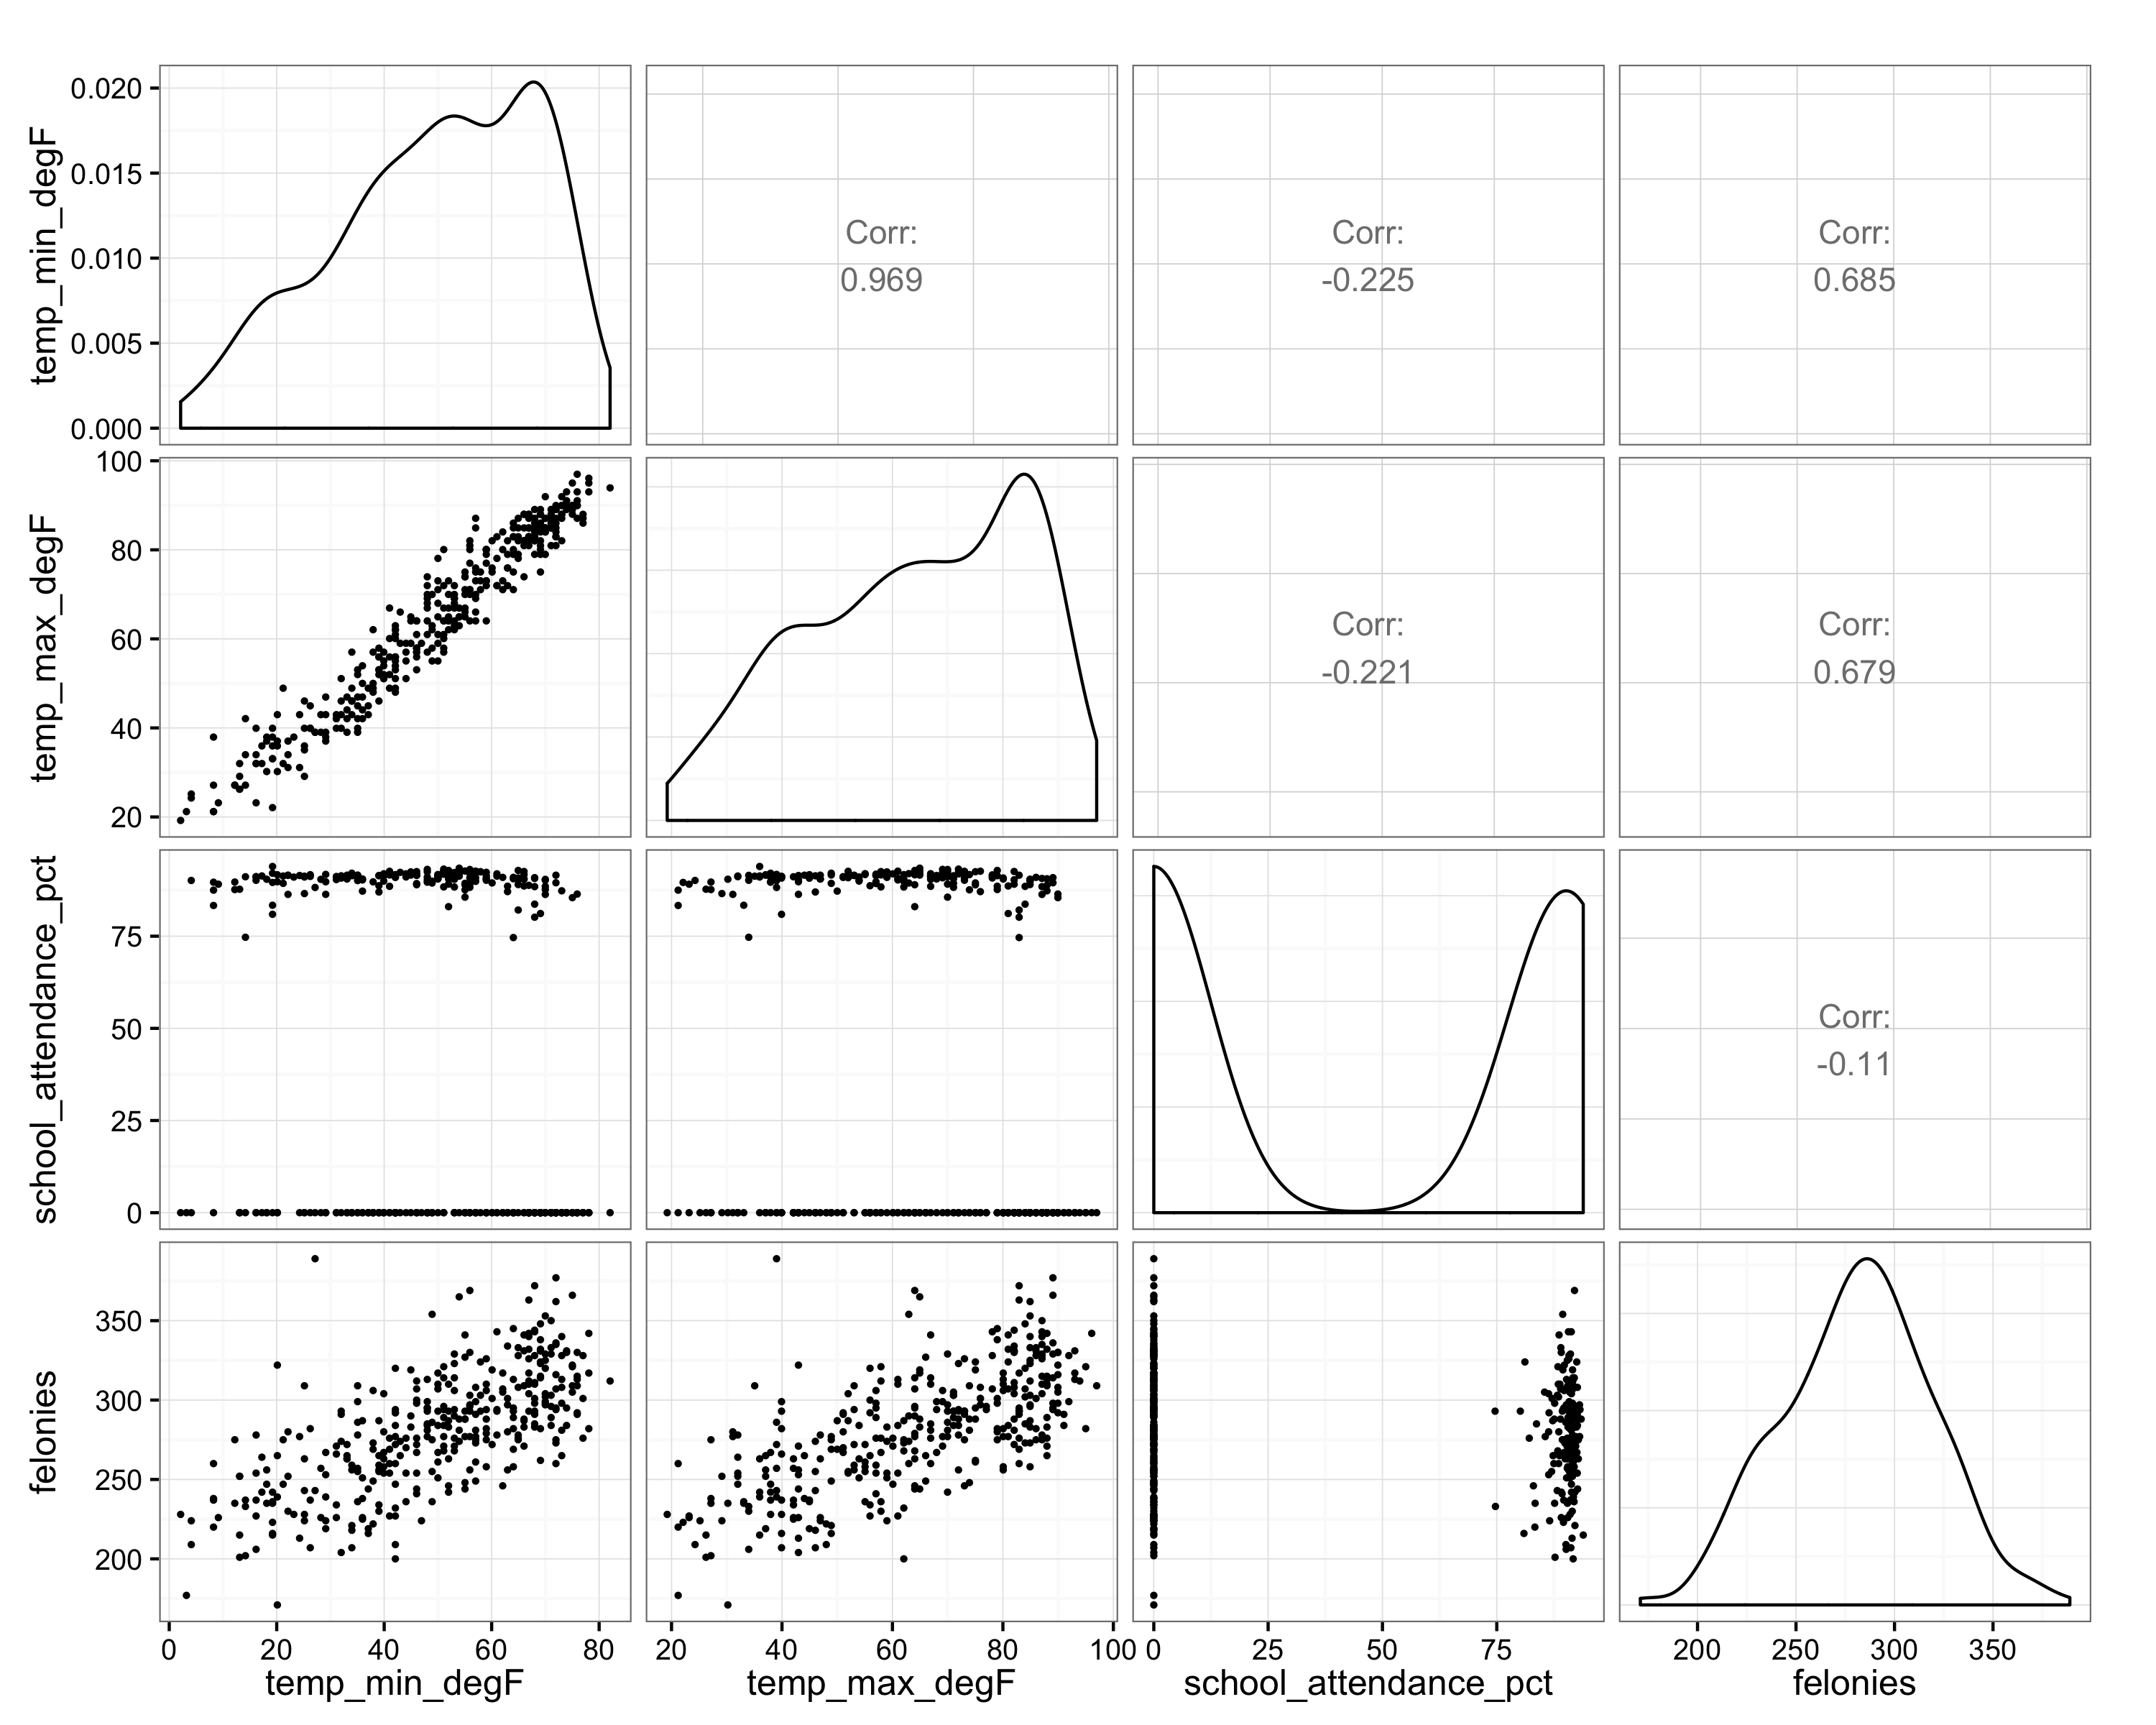
\includegraphics[width=6in]{figures/pairsNumericExclAcc.png}
	\caption{Pairwise scatterplots of some of the numeric variables in the raw dataset.}
	\label{fig:pairsNumericExclAcc}
\end{figure}

From this figure we first notice that there are approximately linear relationships between \texttt{felonies} and \texttt{temp_min_degF}, and between \texttt{felonies} and \texttt{temp_max_degF}. There is also strong collinearity between \texttt{temp_min_degF} and \texttt{temp_max_degF} (correlation: 0.969), however, so we remove one of these variables (\texttt{temp_max_degF}) from the covariates that will be used in the regression model.

Figure \ref{fig:pairsNumericExclAcc} also shows that there is no linear relationship between \texttt{felonies} and \texttt{school_attendance_pct} (the percent of students present in school on a given day). Any non-school-day has 0\% attendance, so instead of using this as a numeric variable, we convert it to the indicator variable \texttt{is_school_day}, taking value ``1'' if NYC Public Schools were open and in session on the given date (i.e., if \texttt{school_attendance_pct} is $>0$), or value ``0'' otherwise.

Faceted boxplots of the categorical variables are shown in Figure \ref{fig:facetCategorical}.

\begin{figure}[!h]
	\centering
	\captionsetup{width=0.9\textwidth}
	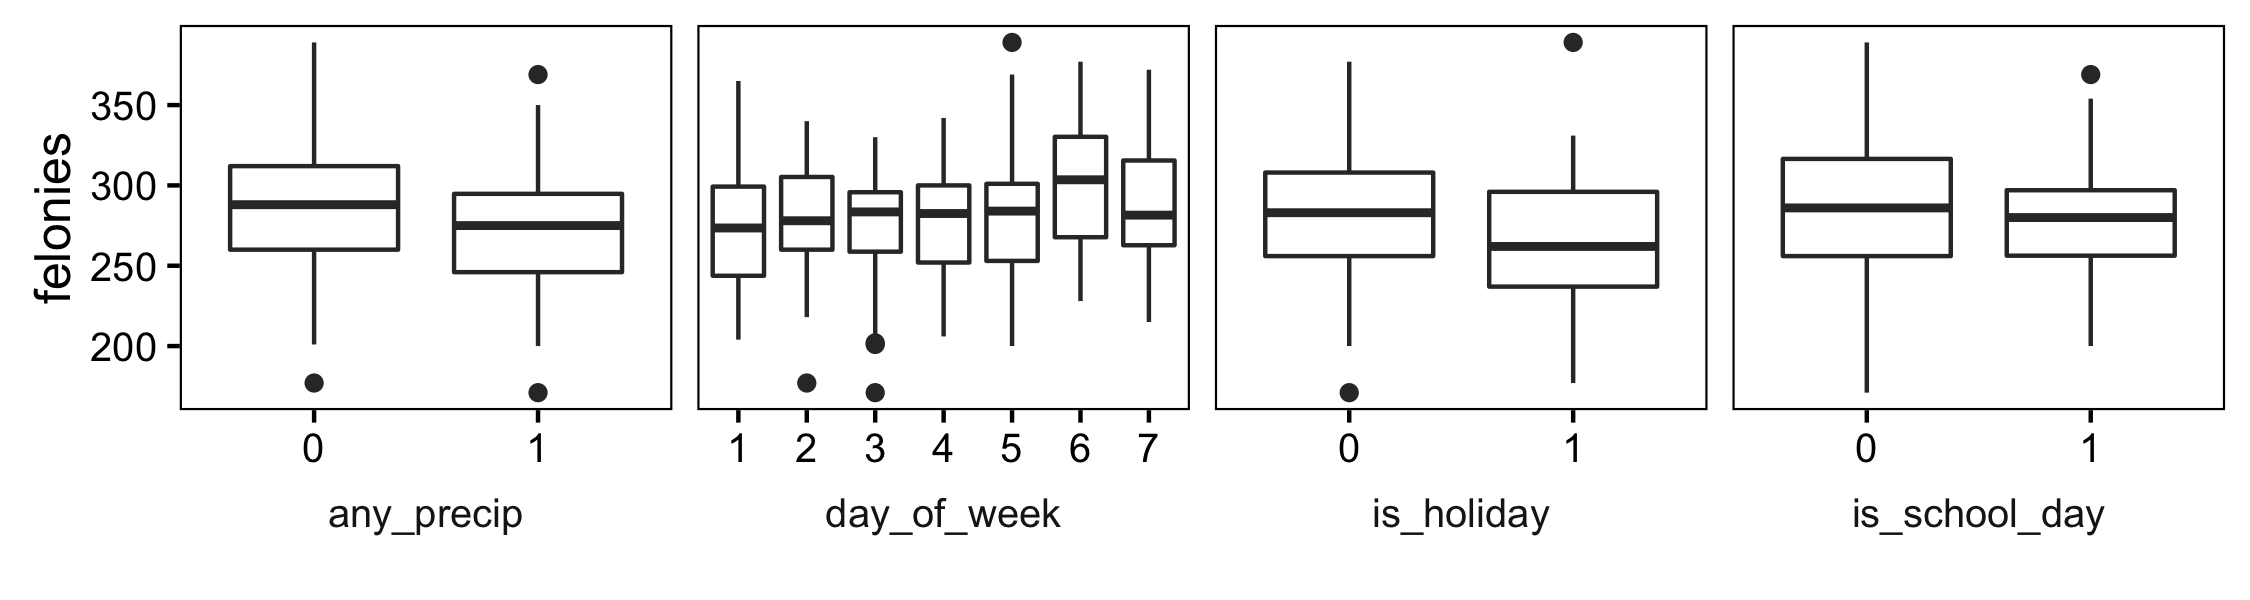
\includegraphics[width=6in]{figures/facetCategorical.png}
	\caption{Faceted boxplots of the categorical variables in the dataset.}
	\label{fig:facetCategorical}
\end{figure}

A Q-Q plot of \texttt{felonies} in Figure \ref{fig:qqFelonies} shows that the variable isn't perfectly normally distributed, but that normality is a reasonably good assumption.

\begin{figure}[!h]
	\centering
	\captionsetup{width=0.9\textwidth}
	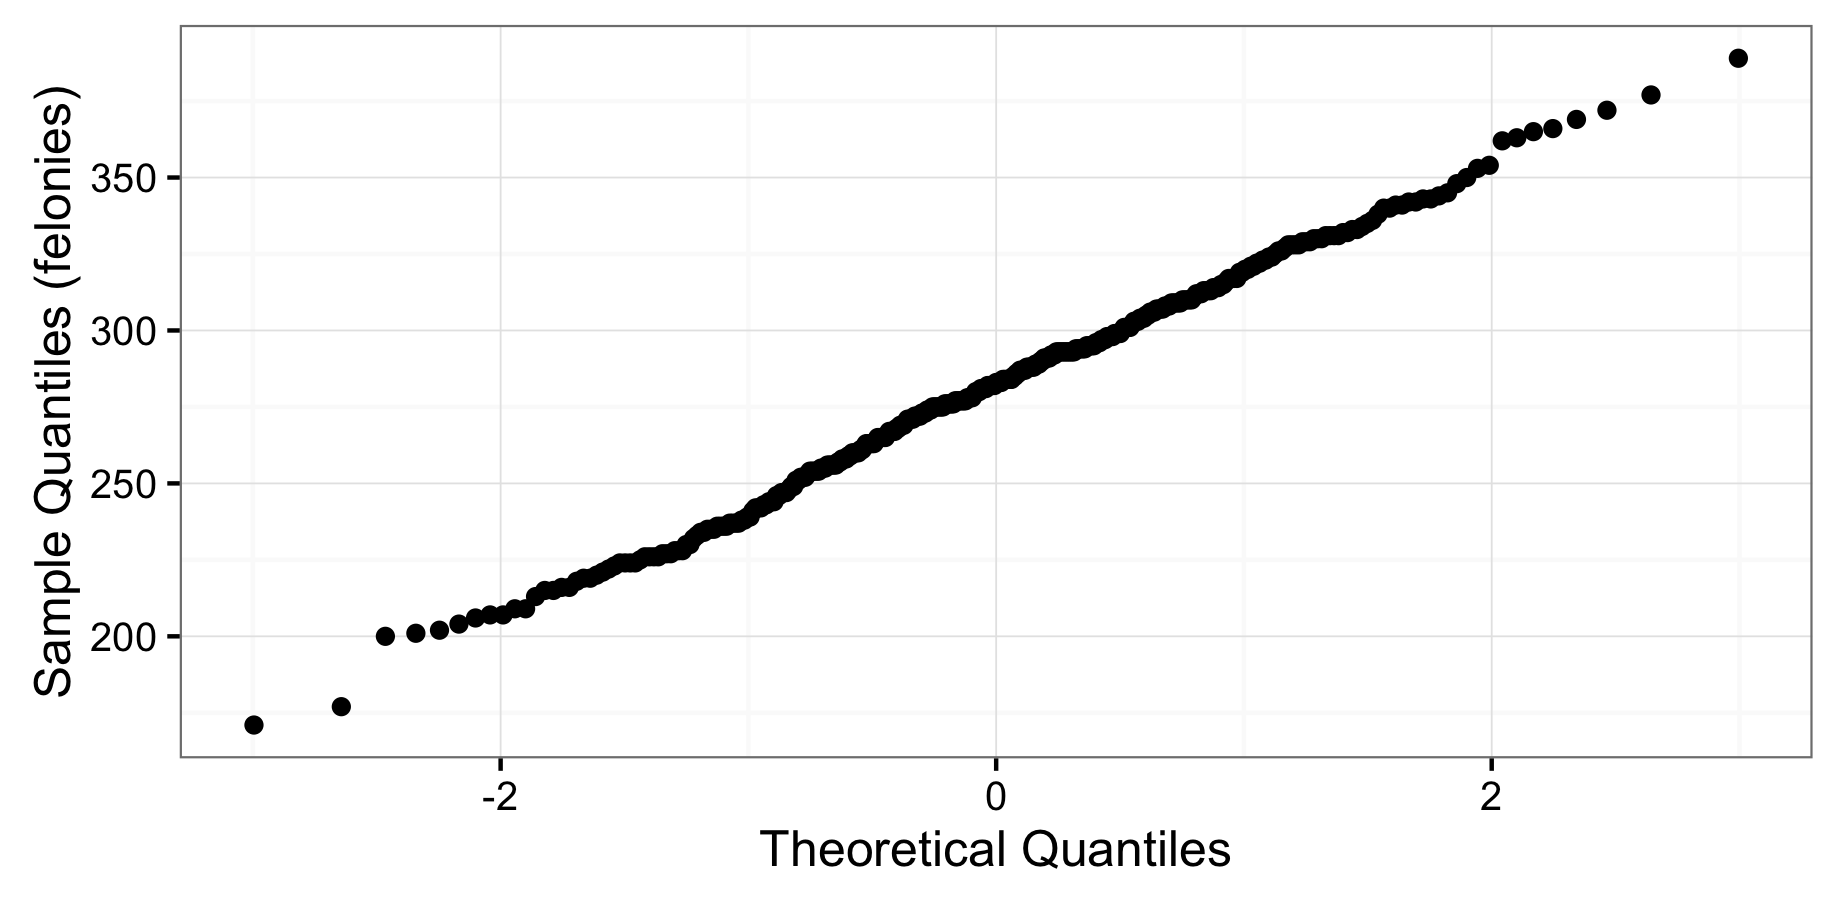
\includegraphics[width=4in]{figures/qqFelonies.png}
	\caption{Faceted boxplots of the categorical variables in the dataset.}
	\label{fig:qqFelonies}
\end{figure}




\section{statistical model and statistical analysis}


\subsection{model setup: the statistical model employed and assumptions}
\label{sec:linearRegressionModelAndAssumptions}


\subsection{statistical analysis / inference}
\label{sec:statisticalAnalysisAndInference}






\section{model checking (and model improvement if the originally proposed model is not appropriate)}
\label{sec:modelChecking}






\section{Conclusion}
\label{sec:conclusion}





\pagebreak

% To compile the bibliography: BibTeX, PDFLaTeX, Quick Build.
%\nocite{*} % This command includes all sources to be listed in the bibliography, even if uncited in the article.
%\singlespacing
%\bibliographystyle{unsrt}
%\bibliography{bib_name}

\end{document}

